\documentclass{article}\usepackage[]{graphicx}\usepackage[]{color}

\usepackage{alltt}
\usepackage{float}
\usepackage{graphicx}
\usepackage{tabularx}
\usepackage{siunitx}
\usepackage{amssymb} % for math symbols
\usepackage{amsmath} % for aligning equations
\usepackage{textcomp}
\usepackage{booktabs}
\usepackage{mdframed}
\usepackage{natbib}
\usepackage[colorinlistoftodos]{todonotes} % to make comments on the margin
\usepackage[small]{caption}
\setlength{\captionmargin}{30pt}
\setlength{\abovecaptionskip}{0pt}
\setlength{\belowcaptionskip}{10pt}
\topmargin -1.5cm        
\oddsidemargin -0.04cm   
\evensidemargin -0.04cm
\textwidth 16.59cm
\textheight 21.94cm 
%\pagestyle{empty} %comment if want page numbers
\parskip 7.2pt
\renewcommand{\baselinestretch}{1.5}
\parindent 0pt
%\usepackage{lineno}
%\linenumbers

%% R Script

\title{Woody plant phenological responses are strongly associated with key functional traits- Outline}

\begin{document}

\maketitle

\noindent Authors:\\
The Wolkovich Lab in 2021 $^{1,2,3,4}$
\vspace{2ex}\\
\emph{Author affiliations:}\\
$^{1}$Forest \& Conservation Sciences, Faculty of Forestry, University of British Columbia, 2424 Main Mall, Vancouver, BC V6T 1Z4;\\
$^{2}$Arnold Arboretum of Harvard University, 1300 Centre Street, Boston, Massachusetts, USA;\\
$^{3}$Organismic \& Evolutionary Biology, Harvard University, 26 Oxford Street, Cambridge, Massachusetts, USA;\\
$^{4}$Edificio Ciencias, Campus Universitario 28805 Alcalá de Henares, Madrid, Spain\\
 

\vspace{2ex}
$^*$Corresponding author: deirdre.loughnan@alumni.ubc.ca\\
\renewcommand{\thetable}{\arabic{table}}
\renewcommand{\thefigure}{\arabic{figure}}
\renewcommand{\labelitemi}{$-$}
\setkeys{Gin}{width=0.8\textwidth}

Climate change is altering the timing of species phenologies, with changes in temporal niches reshaping ecological communities and interactions between species. In temperate systems, the observed advances in plant phenological events, such as budburst, leafout, and flowering times, are associated with changes in seasonal temperatures, particularly warming winter and spring conditions \citep{Menzel2006,Fitter2002}. But despite this strong general trend, phenological responses vary across species and geographically, and we have yet to fully understand the underlying mechanisms driving observed differences \citep{Chuine2010,Morin2009}. As the effects of climate change become more pronounced, understanding these relationships is of increasing importance if we are to predict and preserve the diversity and services found in temperate forest ecosystems. %The relationships between environmental cues and phenological events define for example, the duration of the growing season, the trajectory of community assembly, species ranges, and ecosystem services \citep{Cleland2007,Lopez2008,Chuine2010}, ultimately shaping and mitigating the impact of climate change on forest communities.

While we have yet to identify all drivers of selection on phenologies, considerable work has shown the importance of three abiotic cues -- chilling, forcing, and photoperiod -- as the primary drivers of budburst and leafout in temperate deciduous species \citep{Basler2014,Chuine2016, Harrington2016,Flynn2018}. For budburst to occur, species must experience extended period of cold temperatures to break dormancy \citep{Cooke2012}, where species with higher chill requirements budburst later in the season. Spring forcing temperatures, or the temperatures needed to cue species to initiate growth after dormancy release, are also changing as temperatures warm and the timing at which suitable temperature thresholds are met occur earlier within the season (citation). Photoperiod cues can also determine a species ability to initiate growth \citep{Basler2014,Zohner2020}. Species with strong photoperiod requirements are, however, expected to be more constrained in their ability to track changes in temperature and may face fitness costs and novel species interactions as a result \citep{Guy2014, others?}. Previous studies support the general trend of advancing budburst in response to each cue, but with considerable variation in the relative importance of different cues across species \citep{Chuine2016,Flynn2018}. Some woody plant species, for example, require less forcing to budburst after experiencing a cool winter with more chilling, while also having the ability to compensate for low chilling with high forcing conditions or longer photoperiods \citep{Laube2014,Harrington2015,Flynn2018,Caffarra2011,Basler2014,Zohner2016}. Evidence for the role of photoperiod is largely species specific  \citep{Heide1993, Basler2014, Singh2017, Zohner2016}, with few studies testing for its importance across species in a community (but see  \cite{Flynn2018}). Species that are less dependent on photoperiod cues and able to track trends in temperatures may benefit from greater intra-annual phenotypic plasticity resulting in greater fitness outcomes under increasingly variable climates (citation?). Despite the insights that identifying these proximate drivers have provided, we still lack a generalizable and mechanistic understanding of why species and populations differ in their cue use that. Further insight on this topic is needed to predict future changes in species sensitivities and community structure.\\

In our efforts to understand variation in spring phenological timing, researchers have tested several potential mechanisms to identify the drivers of species cue responses. Work exploring drivers of intraspecific cue use, for example, has found age or the development stage of woody plants to be important. Younger life stages, including both seedlings and younger understory trees, both budburst earlier than mature individuals in the canopy \citep{Vitasse2013,Seiwa1991}. These trends reflect both differences in the temperature sensitivities across life stages and effects of ontogenic changes as trees mature \citep{Vitasse2013,Seiwa1991}. Interspecific differences in cues, however, have been studied in relation to species' phylogenetic relatedness. Work on this topic has found strong evidence for events like flowering-time and budburst to be consistent within taxonomic families, suggesting conservatism in the genetic and physiological mechanisms that determine species phenologies \citep{Kochmer1986,Davies2013,Gougherty2018}. Studies of woody plant phenologies across species ranges have also highlighted the importance of local adaptations, with the presence of gradients in phenological responses and presumably cue use at northern range limits \citep{Lechowicz1984,Chuine2001,Chuine2010}. In temperate systems for example, greater temperature variation in North America was associated with higher chilling requirements and more conservative phenological responses \citep{Zohner2017}.  Studies testing for trends in cues responses across species latitudinal ranges have also observed stronger responses to photoperiod cues at lower latitudes \citep{Zohner2016}. Exploring these potential drivers of plant phenologies have illustrated the nuanced nature of phenology in shaping diverse communities, but they are still limited in the degree to which they explain the variation we observe across species and ecosystems.\\

Taking a functional trait approach to phenological research could help explain the variation in cue use across species and geographically \citep{Flynn2018,Osada2017}. Early work on functional traits used trait data from diverse global assemblages of deciduous plants to identify associations between traits, common growth strategies, and different niche space \citep{Westoby1998,Wright2004,Chave2009}. The resulting leaf-height-seed scheme and the more extensive leaf economic spectrum found direct associations between several trait values and gradients in species growth rates and competitive abilities \citep{Westoby1998,Wright2004,Diaz2016,Chave2009,Funk2016}. While reproductive phenological traits have been identified as ecologically important for many years \citep{Weiher1999, Laughlin2014}, few studies have explored their role in the larger trait framework. Spring phenological traits, such as budburst and leafout, define the beginning of the growing season and period of photosynthesis, and therefore also have the potential to correlate with established growth strategies. Support for the existence of trade-offs in budburst dates and traits related to growth and resource use have been observed across plant functional groups and habitat types in a handful of studies. For example, several studies have found deciduous woody species with smaller vessel diameters and diffuse or semi-ring-porous xylem structures to leaf out earlier than species with larger vessels, as this anatomy reduces the risk of embolism during freezing events  \citep{Panchen2014, Lechowicz1984}. In testing relationships between budburst and leaf traits of deciduous tree species in Japan, \citep{Osada2017} found positive correlations between budburst date and leaf area, leaf mass, and nitrogen content by both mass and area, while \citep{Sun2006} found deciduous species with high leaf mass per area (a trait that is the inverse of specific leaf area) to budburst earlier in deciduous oak forests in eastern China. %Note their prediction is opposite ours 
Variation in leafout can also relate to species heights, both intraspecifically and across functional groups, with shorter individuals or understory species leafing out earlier than taller individuals or canopy species \citep{Seiwa1998, 1999b}. To date, however, research in this area has focused on individuals at local scales, or few traits for a small number of species, limiting our ability to draw more general and causal inferences. There is also a lack of studies linking traits directly to cue sensitivity rather than phenological date. The likely associations between cue sensitivity, phenological events, and growth strategies may allow for more generalizable trends across species and sites, and better account for species variability in key environmental cue use. \\


%Studies of flowering phenology in herbaceous species also find phenology to relate to commonly measured traits, with early germinating species being taller with greater relative growth rates than later germinating species \citep{Sun2011}. 

% Faith commented that the first two sentences below are repetitive 
To date, there have been numerous studies investigating the relationships between climate and functional traits and a wealth of literature on the separate effects of climate cues as drivers of phenology. However, the selective pressures shaping species traits under variable temperatures are also likely to act on species responses to phenological cues and define a species temporal niche. Species with a more acquisitive life-strategy have shorter rates of return on resource investments and the ability to take advantage of the greater abundance of soil nutrients and light early in the growing season. Such species face a lesser cost in initiating phenological events too early, as they can recover from early season damage (Cat's paper?). For example, some acquisitive species produce leaves with high leaf nitrogen content and Specific Leaf Area (SLA) and can take advantage of greater light availability by having higher rates of photosynthesis \citep{Wright2004,Pereira2020}, while also limiting the costs of tissue production \citep{Lambers2004, Westoby2006, Herault2011}. Acquisitive-strategy species also invest less in their wood structure, having lower heights and stem densities \citep{Laughlin2010}. Species that budburst earlier in the growing season require less spring forcing and winter chilling, and shorter photoperiods \textbf{(cite Flynn \& Wolkovich, 2018)}, allowing them to grow under less competition for light and soil resources. The suite of traits of acquisitive species contrasts with more conservative life-strategy species that exhibit slower, more competitive growth strategies that benefit from slower rates of return on resource investment and the longer retention of leaf tissue. A greater requirement for cue unit accumulation to trigger phenological events should align with a more conservative life-strategy as such species seek to avoid damage due to premature development.      
 
% Hmmm... is this paragraph still relying heavily on early/late narative?
   
In this study, we test for associations between plant phenological responses to environmental cues and common functional traits. Budburst data for tree species in controlled environmental studies was selected from the Observed Spring Phenology Response in Experimental Environments (OSPREE) database and paired with functional trait data from the TRY and BIEN databases. This data was used to explicitly test for the relative differences in functional traits and the timing of budburst in response to experimental forcing, chilling, and photoperiod cues. Drawing on previous work and the broader trait literature, we predict that species that respond less strongly to chilling, forcing, and photoperiod conditions are more likely to have traits associated with acquisitive growth but low competitiveness, as reflected by high SLA, high LNC, shorter heights, and lower seed mass. In contrast, species that are more responsive to chilling, forcing and photoperiods will have traits more associated with conservative growth and higher competitive abilities, such as low SLA, low LNC, greater heights and heavier seeds. 


\begin{figure}[h!]
    \centering
 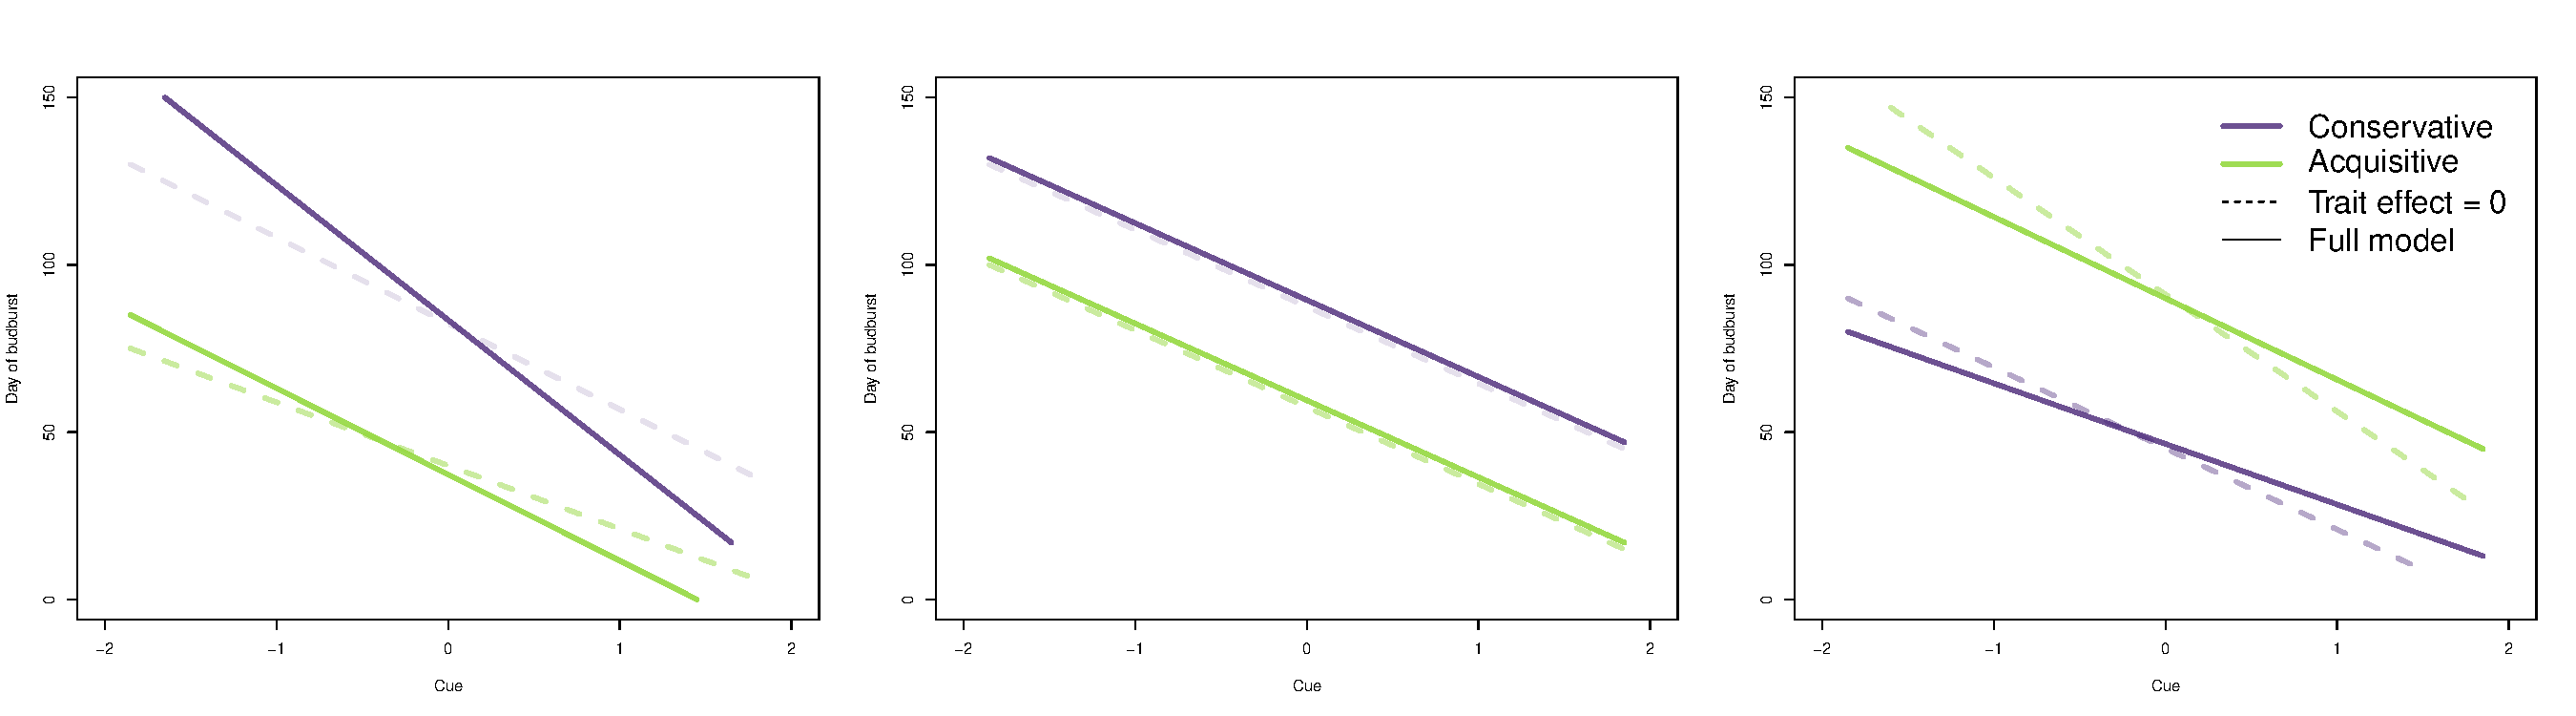
\includegraphics[width=\textwidth]{..//..//analyses/traits/figures/conceptFig.pdf} 
    \caption{Conceptual figures}
    \label{config}
\end{figure}

Using tree height as an illustrative example, we predict taller trees to be more conservative in their growth strategies and shorter species to budburst earlier and exhibit a more acquisitive growth strategy. Previous work on cue responses in woody species have consistently observed negative responses to stronger cues, resulting in advanced budburst, and therefore we predicted that the estimated cue responses from our models would all be negative. Under this assumption, there could be three possible trends in the relationships between cue and trait effects on budburst date. If phenological responses are in line with trait variation associated axes of acquisitive to conservative growth, we predict there to be a complimentary %what term works best? Supplemental? Additive? Increasingly negative?
 trait effect on cue responses (Fig 1a). This would result in a negative trait effect, resulting in a steeper slope in the cue response and a stronger cue response and advance in budburst dates with higher cues. This is illustrated by the steeper slope of the solid lines for both the conservative and acquisitive species in Figure 1a. The more conservative species also exhibits later budburst dates than the more acquisitive species. The smaller differences in slopes for the cue only and full model observed for species with low traits is due to the magnitude of the trait value and not a difference in strength of the response. If other functional traits have no relation to budburst phenology, the trait effect will be estimated as zero and we could expect to see no difference in the slopes of full model and cue only model (Fig 1b.). Finally, if our model estimates a positive trait effect, potentially as a result is a trade-off in selection for budburst phenology and resource use or competitiveness, we predict the slopes of our full model to be less steep than the cue only model (Fig 1c). We may also see less acquisitive species having later budburst dates than species with traits associated with conservative growth strategies (Fig 1c.

\section{Methods}
For our analysis, we combined phenological data from the OSPREE database \citep{OSPREE} with functional trait data from the TRY(cite) and BIEN (cite) trait databases. 

%describe OSPREE breifly
The OSPREE database contains woody, deciduous species phenological data for which experimental data on phenological cues is available, and for which the phylogenetic relationship is well known. First published in 2019, this database has since been updated, and now includes the review of an additional 623 and 270 new publications from each search term respectively. From this subsequent review, we added an additional 12 papers. For additional information on the construction of the OSPREE database and methods of cue estimates, see \citep{OSPREE}. Our analysis used all available budburst data for our 37 focal species, with the data originating from 28 unique studies. 

%Describe TRY and BIEN breifly 
Both TRY and BIEN are large databases compiling plant trait data across many individuals, species, and studies. Initially, we began by selecting height, seed mass, LNC, SLA, stem specific density (SSD) and leaf dry matter content (LDMC) data for all 234 species represented in the OSPREE database.  

%Trait data for ten functional trait was requested from the TRY databases for all 96 species (Table S1 - table of requested traits for each database). Additional trait data was acquired from the BIEN database using the BIEN R package (version X). From the BIEN database we obtained data for 34 species and seven species (Table S1). 

We began by searching for trait data for all 234 species represented in the OSPREE database. Data was also obtained from the BIEN database using the BIEN R package \citep{Maitner2017}. Data was requested or downloaded in December 2018. Our full trait datasets included data on x species .... (S Table x - a table only showing trait data for traits we actually used. Not all the ones we requested.) 

For our analysis we only included trait data from adult individuals with a minimum height of 1.42 m and we removed all data from experiments or growing in non-natural habitats. Traits were also grouped where appropriate, for example, separate entries for specific leaf area (SLA) values with petioles, without petioles, and for which no petiole presence was specified were all categorized as a single trait in our analysis (see Table S1). Duplicated data across the datasets were removed (n= 434905). Finally, we subsetted the data to include only species for which we had a complete dataset for each species and trait. This resulted in a dataset of only 26 species and six functional traits. To test for correlations in our six traits and further refine our trait selection, we performed a PCA. The principle component explained 32.2\% of variation while the second explained 23.4\% of the variation (Fig. S1). Given the strong association between the SLA and LDMC leaf traits, and similarly between stem specific density (SSD) and height, we further reduced the number of traits in our analysis to include only height, seed mass, LNC, and SLA. By including only these four traits, we had at least one trait measurement for 37 species (height n = 47781, seed mass n = 281, LNC n = 3853, SLA n = 7656). Given the abundance of height data and overrepresentation of height measurements for six of our focal species, we randomly sampled 3000 height measurements for each of these species to include in our analysis (n = 27318). This reduces the effect of trait values from these frequently measured species from overwhelming the partial pooling effect in our model. In addition we excluded seed mass data from the HE Marx dataset from BIEN, as it consisted of only one value, making it challenging to include the study level effect in our model\\ 

To test the relationships between functional traits and species cue responses, we developed a joint hierarchical bayesian model. Our model is composed of two sub-models that are co-estimated and linked by shared parameters. Because each trait varied in the number of studies in which it is included as well as the number of individuals for which it is measured, we chose to model each trait separately. The first part of the model is a hierarchical intercept only model (Equations \ref{TraitsLine_main}, \ref{TraitsLine_sp} \& \ref{TraitsLine_study}) estimating species mean trait value for species $i$ ($trait_{i}$). This ($trait_{i}$) value is a combination of a species mean trait value $\alpha_{sp,i}$ and a hierarchical grouping term on the intercept for study to account for study level differences in the trait data ($\alpha_{study,i}$).  \\

The second part of our models is a hierarchical linear model (Equation \ref{phen_main}) regressing the date of budburst $b$  ($pheno_{b}$) against a combination of chilling, forcing and photoperiod units. To explicitly compare the effects of chilling, forcing, and photoperiod, we used standardized z-scored values for the predictor variables which accounts for the differences in the scale of predictors across studies \citep{Gelman2006}, as well as the natural units for the cues (including chill units, $^\circ$C, and hours for chilling, forcing, and photoperiod respectively). We test whether there is a link between phenological cue response ($\beta chill_{sp}$,$\beta force_{sp}$,$\beta photo_{sp}$) and mean traits by including the mean trait values from the previous model ($\alpha_{sp}$) in the estimation of the cue slopes. Each cue slope is a combination of a species-specific slope value ($\alpha cue$) independent of trait, and the species trait value ($\alpha_{sp}$) (Equations \ref{alphachilleq}, \ref{alphaForceq} \& \ref{alphaPhotoeq})multiplied with an interaction parameter $\beta trait.cue$ (Equations \ref{betaChillEq}, \ref{betaForceEq} \& \ref{betaPhotoEq}). A greater $\beta trait.cue$ value means trait is more strongly related to cue slope, and its sign dictates the direction of the interaction. 

Our model was first developed using test data and our priors validated using prior predictive checks. In our models, we used weakly informative priors, with four simultaneous chains of 1,000 warmup iterations and 2,000 sample iterations. The models produced Rhat values close to 1 and neffs greater than 10\% of the number of iterations %triple check this is true
, indicating that the model performed sufficiently well.  We fit our models using the Stan programming language (Stan citation), interfaced with using the rstan package (version, citation).

%should we define every term in our model so we can be spefiic when we discuss them? I (Faith) usually do this, but our model (models?) is so long!

%Our model uses species-level trait values in our first model to predict species sensitivities to forcing, chilling, and photoperiod experimental cues. In addition to including partial pooling across species, the trait portion of the model includes a study level effect, thereby accounting for not only differences across species, but also the effects of methodological differences, and differences across habitats. The first model in our analysis calculates the latent variable that is then incorporated into the second phenology model. Values close to zero reflect small relationships between traits and cues values, while greater values represent high correlations between traits and phenological cues. This model was developed and validated using test data.{}
 
 % How much detail is needed - justify our approach or just include the model?
 %Do we include code for combining the effect of the grand mean with the species level effect?

\begin{equation}
\label{TraitsLine_main}
trait_{i} \sim N( \alpha_{sp,i} + \alpha_{study,i},\sigma_{trait}) 
\end{equation}

\begin{equation}
\label{TraitsLine_sp}
\alpha_{sp} \sim N(\mu, \sigma Sp)
\end{equation}

\begin{equation}
\label{TraitsLine_study}
\alpha_{study} \sim N(0, \sigma Study)
\end{equation} 

\begin{equation}
\label{phen_main}
pheno_{b}  \sim N( \alpha pheno_{sp_b} + \beta force_{sp_b} * Forcing_{b} + \beta photo_{sp_b}  * Photo_{b} + \beta chill_{sp_b} * Chill_{b} , \sigma_{pheno} ) 
\end{equation} 

\begin{equation}
\label{betaChillEq}
\beta chill_{sp} = \alpha chill_{sp} + \beta trait.chill * \alpha sp_{sp}
\end{equation} 

\begin{equation}
\label{betaForceEq}
\beta force_{sp} = \alpha force_{sp} + \beta trait.force * \alpha sp_{sp}
\end{equation} 

\begin{equation}
\label{betaPhotoEq}
\beta photo_{sp} = \alpha photo_{sp} + \beta trait.photo * \alpha sp_{sp}
\end{equation}

\begin{equation}
\label{alphaPheneq}
\alpha pheno  \sim N(\mu_{pheno}, \sigma_{pheno}) 
\end{equation}

\begin{equation}
\label{alphaForceq}
\alpha force \sim N(\mu_{force}, \sigma_{force}) 
\end{equation}

\begin{equation}
\label{alphachilleq}
\alpha chill  \sim N(\mu_{chill}, \sigma_{chill})
\end{equation}

\begin{equation}
\label{alphaptotec}
\alpha photo  \sim N(\mu_{photo}, \sigma_{photo}) 
\end{equation}

%\begin{align*}
%\hat{trait_i} &= \mu_{grand_{sp}} + \alpha study_{study_i} \\
%\mu_{grand_{sp}} &= \alpha_{grand} + \alpha sp_{sp_i} \\
%\alpha_{grand}  & \sim N(0, \sigma_{grand})\\
%\alpha sp & \sim N(0, \sigma_{sp}) \\
%\alpha study& \sim N(0, \sigma_{study}) \\
%trait_i & \sim N(\hat{trait}_i, \sigma_{trait}) \\
%\vspace{1ex}\\

%\hat{pheno}_i  &= \alpha pheno_{sp_i} + \beta force_{sp_i} * Forcing_{i} + \beta photo_{sp_i}  * Photo_{i} + \beta chill_{sp_i} * Chill_{i} \\
%\beta force_{sp} &= \alpha force_{sp} + \beta trait.force * \alpha sp_{sp}\\
%\beta chill_{sp} &= \alpha chill_{sp} + \beta trait.chill * \alpha sp_{sp}\\
%\beta photo_{sp} &= \alpha photo_{sp} + \beta trait.photo * \alpha sp_{sp}\\
%\alpha pheno & \sim N(\mu_{pheno}, \sigma_{pheno}) \\
%\alpha force& \sim N(\mu_{force}, \sigma_{force}) \\
%\alpha chill & \sim N(\mu_{chill}, \sigma_{chill}) \\
%\alpha photo & \sim N(\mu_{photo}, \sigma_{photo}) \\
%pheno_{i} & \sim N(\hat{pheno_i}, \sigma_{pheno}) \\
%\end{align*}

%As such, we model each trait individually using the same model specified above, but with the appropriate priors for each trait. Priors were tested using prior predictive checks. All analyses were done in Stan (version) using the rstan package (version) in R (version). 

% I wrote this up in case we want to include it
Finally, we used a phylogenetic generalized least-squares regression model (PGLS) to test the relationship between day of budburst and individual traits. This analysis allowed us to test for phylogenetic non-independence in the phenology-trait relationship \citep{Freckleton2002}. We obtained a rooted phylogenetic tree by pruning the tree developed by \citep{Smith2018} and performed the PGLS analysis using the mean trait values and mean posterior estimates of the cue responses from our joint model. The PGLS was run using the "Caper" package in R \citep{Orne2013}. \\

\section{Results}
% I think there are two ways to structure the results - discuss each cue separately or discuss each trait separately - I think each trait is easier and fits our hypotheses better

We estimated mean height as 14m (90\% uncertainty intervals: 11m, 17m). Species height values were distributed with a variance of 6 (90\% uncertainty intervals: 5m, 7m), and study height values were distributed with a variance of 7m (90\% uncertainty intervals: 6m, 9m). The highest estimated mean species height estimate in our dataset was 26m (90\% uncertainty intervals: 22m,29m) for \textit{Quercus petraea}, and the lowest estimated mean height value was 0.7(90\% uncertainty intervals: -2m,4m) for \textit{Rhamnus cathartica}. 

Mean LNC was estimated as 23 (90\% uncertainty intervals: 20, 25). Species LNC values were distributed with a variance of 5 (90\% uncertainty intervals: 4, 7), and study LNC values were distributed with a variance of 4 (90\% uncertainty intervals: 2, 5). The highest estimated mean species LNC estimate in our dataset was 39 (90\% uncertainty intervals: 37,41) for \textit{Prunus persica}, and the lowest estimated mean LNC estimate was 14(90\% uncertainty intervals: 10,17) for \textit{Hamamelis virginiana}.

Mean log$_{10}$ seed mass was estimated as 2.0 (90\% uncertainty intervals:1.5, 2.4), which translates as a seed mass of approximately 104mg. Species log$_{10}$ seed mass values were distributed with a variance of 1.6 (90\% uncertainty intervals: 1.3, 1.9), and study log$_{10}$ seed mass values were distributed with a variance of 0.5 (90\% uncertainty intervals: 0.3, 0.6). The highest estimated mean species log$_{10}$ seed mass estimate in our dataset was 4.2 (90\% uncertainty intervals: 3.9, 4.6) for \textit{Juglans cinerea}, which translates as a seed mass of approximately 18000mg. The lowest estimated mean log$_{10}$ seed mass estimate was -1(90\% uncertainty intervals: -1.4,-0.6) for \textit{Betula populifolia}, which translates as a seed mass of approximately 0.1mg.

We estimated mean SLA as 16.8 (90\% uncertainty intervals:15, 19). Species SLA estimates were distributed with a variance of 8.1 (90\% uncertainty intervals: 6.6, 9.6), and study SLA estimates were distributed with a variance of 3.3 (90\% uncertainty intervals: 1.8, 4.8). The highest estimated mean species SLA estimate in our dataset was 4.9 (90\% uncertainty intervals: 2.9, 6.5) for \textit{Acer pensylvanicum}, and the lowest estimated mean LNC estimate was -1(90\% uncertainty intervals: -1.4,-0.6) for \textit{Quercus coccifera}.

In most cases, the simple geometric mean for each species-trait combination fell within the posterior estimations from our models (Fig. \ref{figure:TraitDistributions}). There were a limited number of species in the height model were the simple geometric mean fell outside of predicted species species means after accounting for the effect of study, for example \textit{Quercus ilex}, \textit{Quercus petraea}, \textit{Quercus coccifera}, and \textit{Aesculus hippocastanum}.


%Our four trait models predicted most species cue responses to be negative, indicating that the average effect of forcing, chilling, and photoperiod cues were to advance budburst date. The exceptions to this were the photoperiod estimates from our height and SLA models, both of which showed a small positive or delaying effect, but considerable variation in the estimated value due to species level differences. The absolute effect of species cue responses was generally greatest for forcing cues, except in our models of LNC, for which chilling cues had the largest absolute response. Photoperiod cues had the smallest cues responses in three of our models, except for our model of tree height, in which the absolute effect of chilling was less than that of photoperiod. The effect of traits on cue responses were all negative and were greatest for forcing and chilling, while the effects of photoperiod cues were weaker across all our models. \\

\begin{figure}[h!]
    \centering
 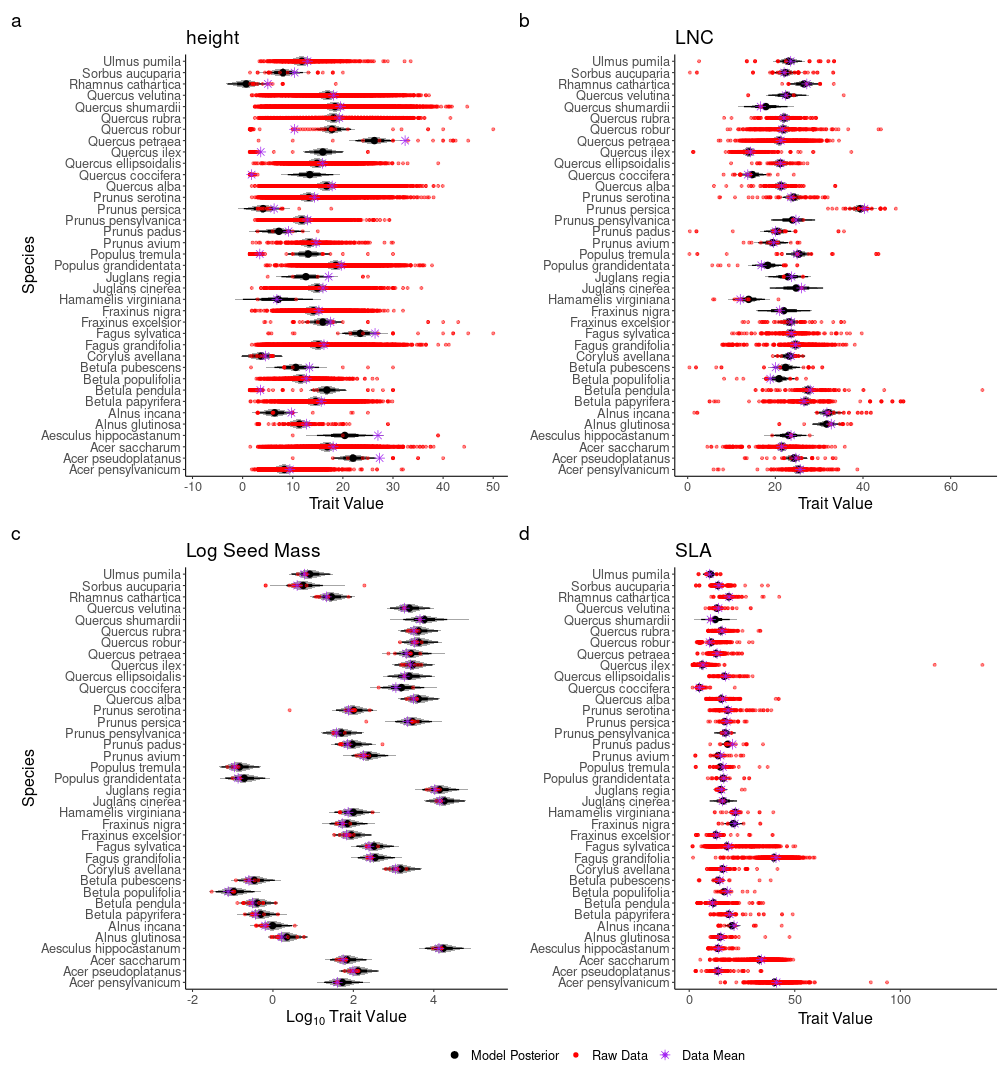
\includegraphics[width=\textwidth]{..//..//analyses/traits/figures/FourTraitFit_37spp.png} 
    \caption{Raw data and posterior esti.}
    \label{figure:TraitDistributions}
\end{figure}

\begin{figure}[h!]
    \centering
 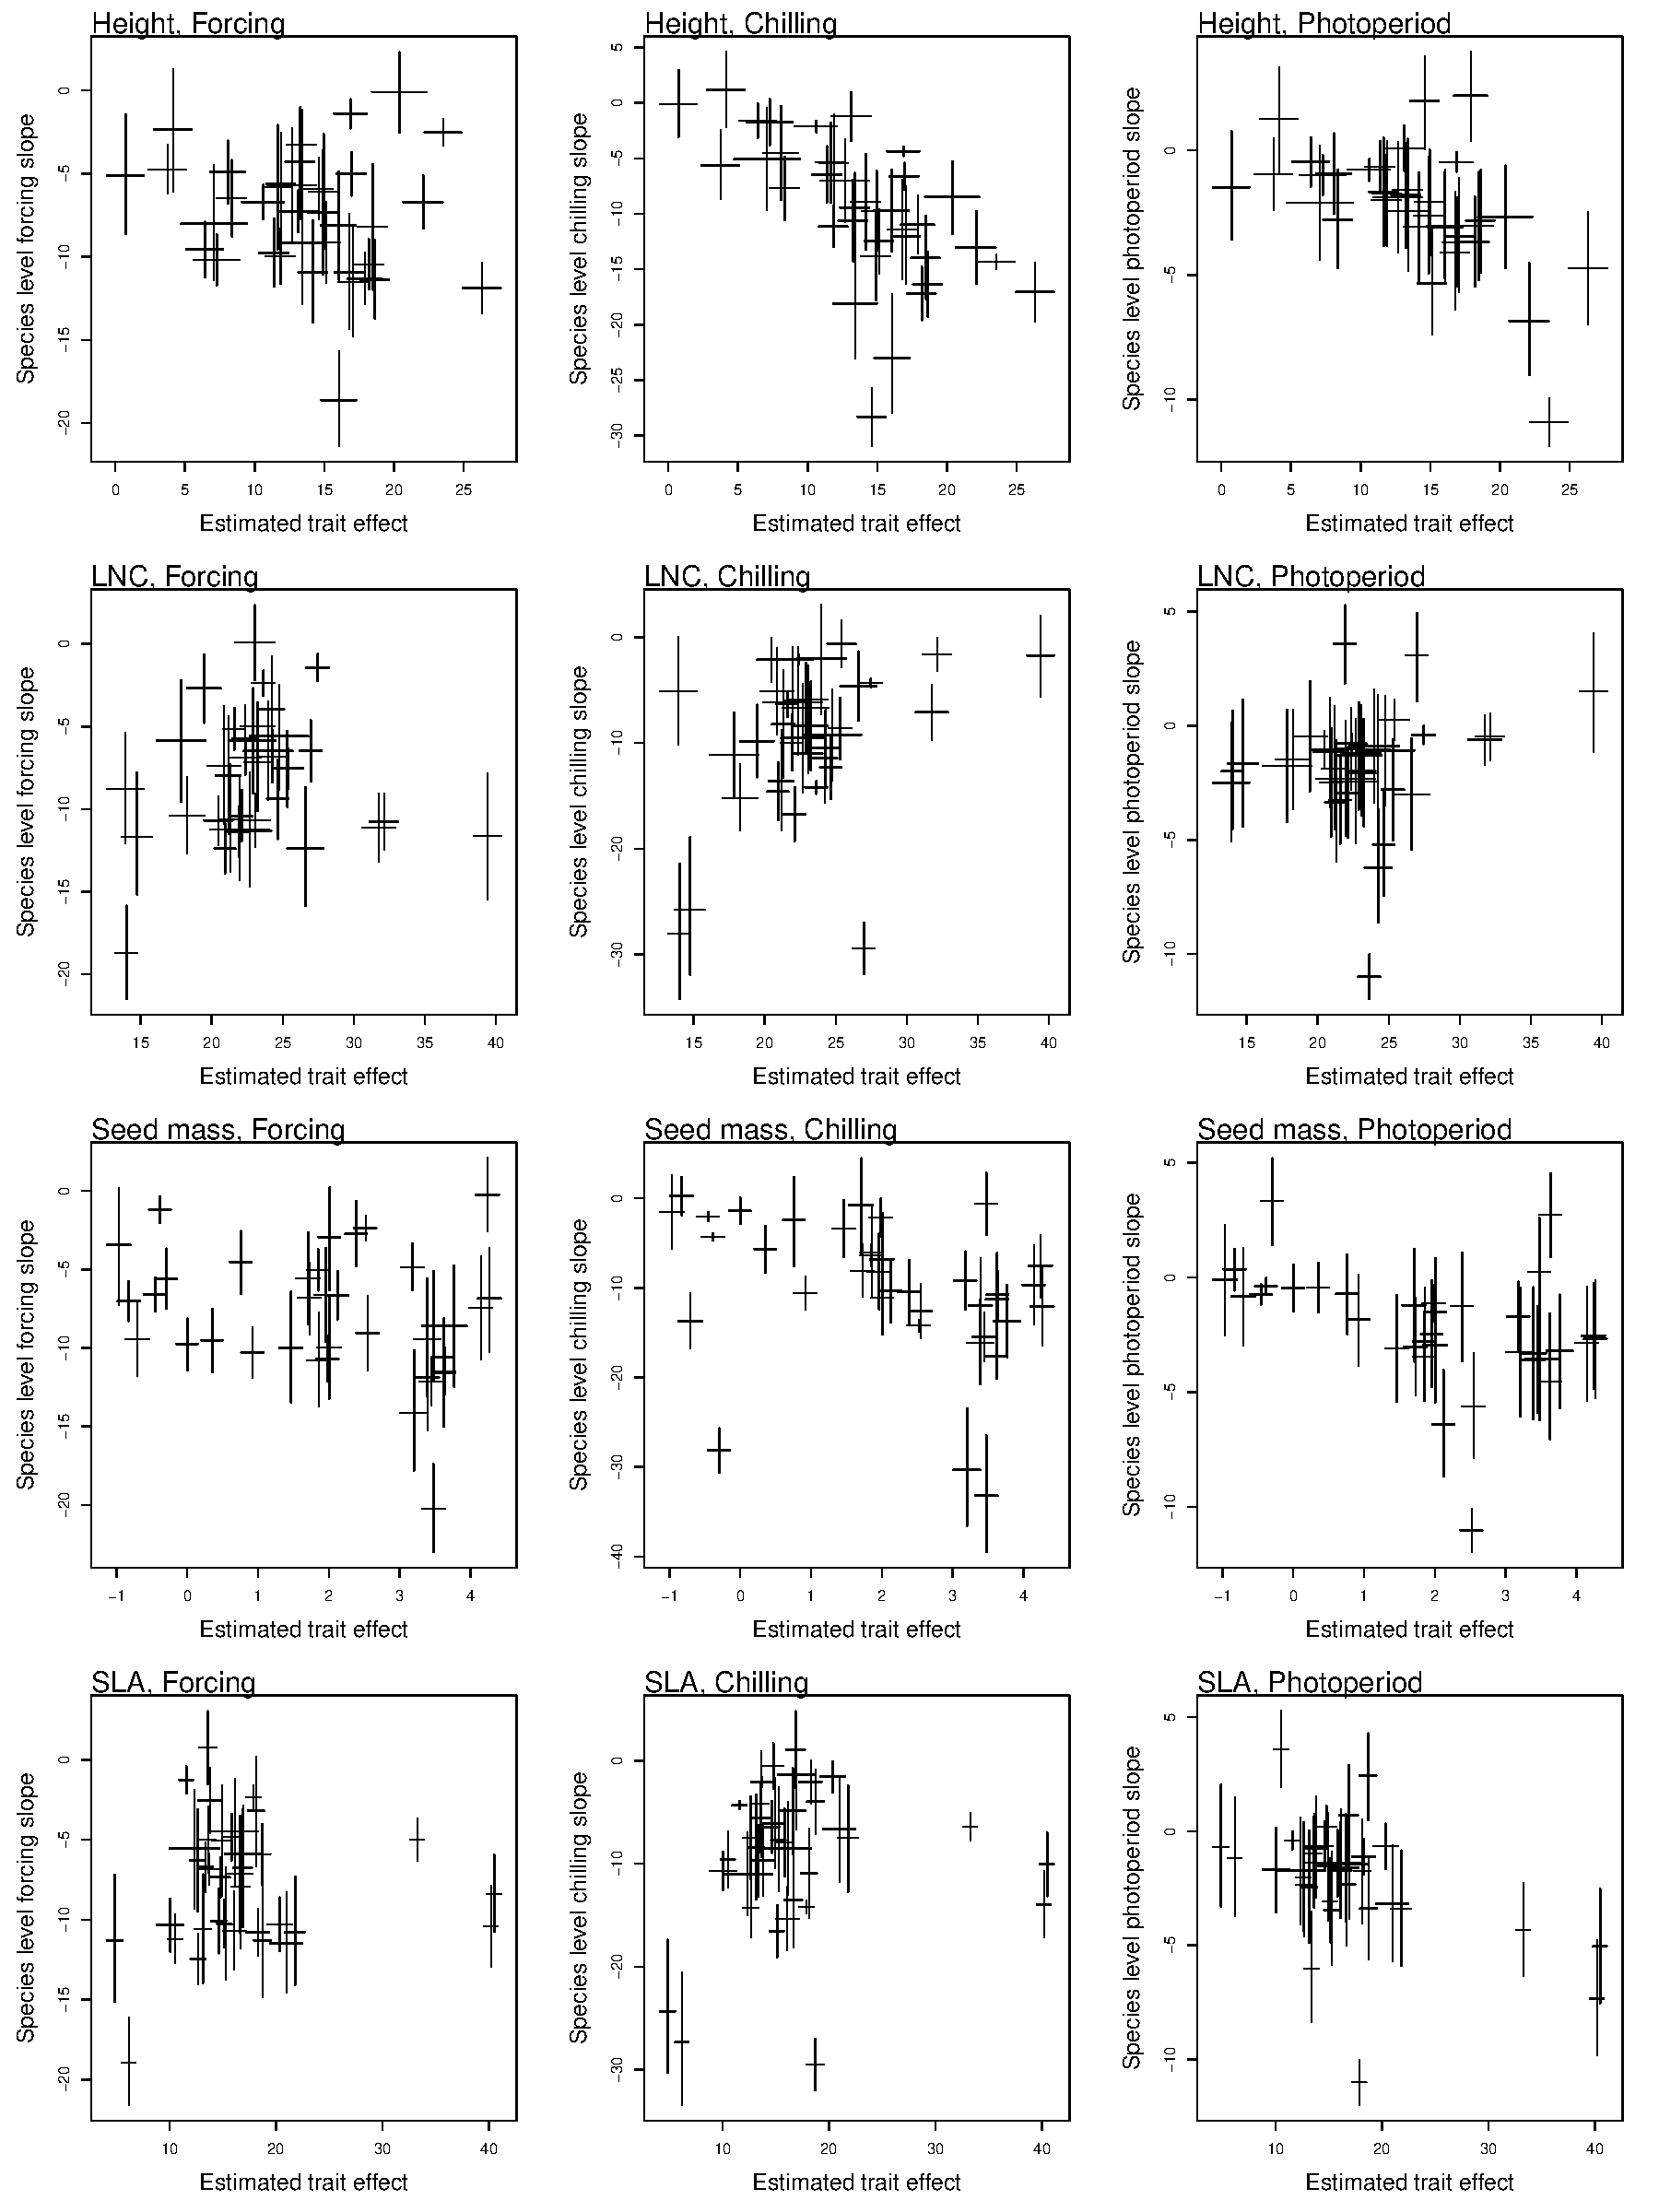
\includegraphics[width=\textwidth]{..//..//analyses/traits/figures/cuetrait.pdf} 
    \caption{Trait relationships with cue slopes}
    \label{fig:cuetraits}
\end{figure}

\begin{figure}[h!]
    \centering
 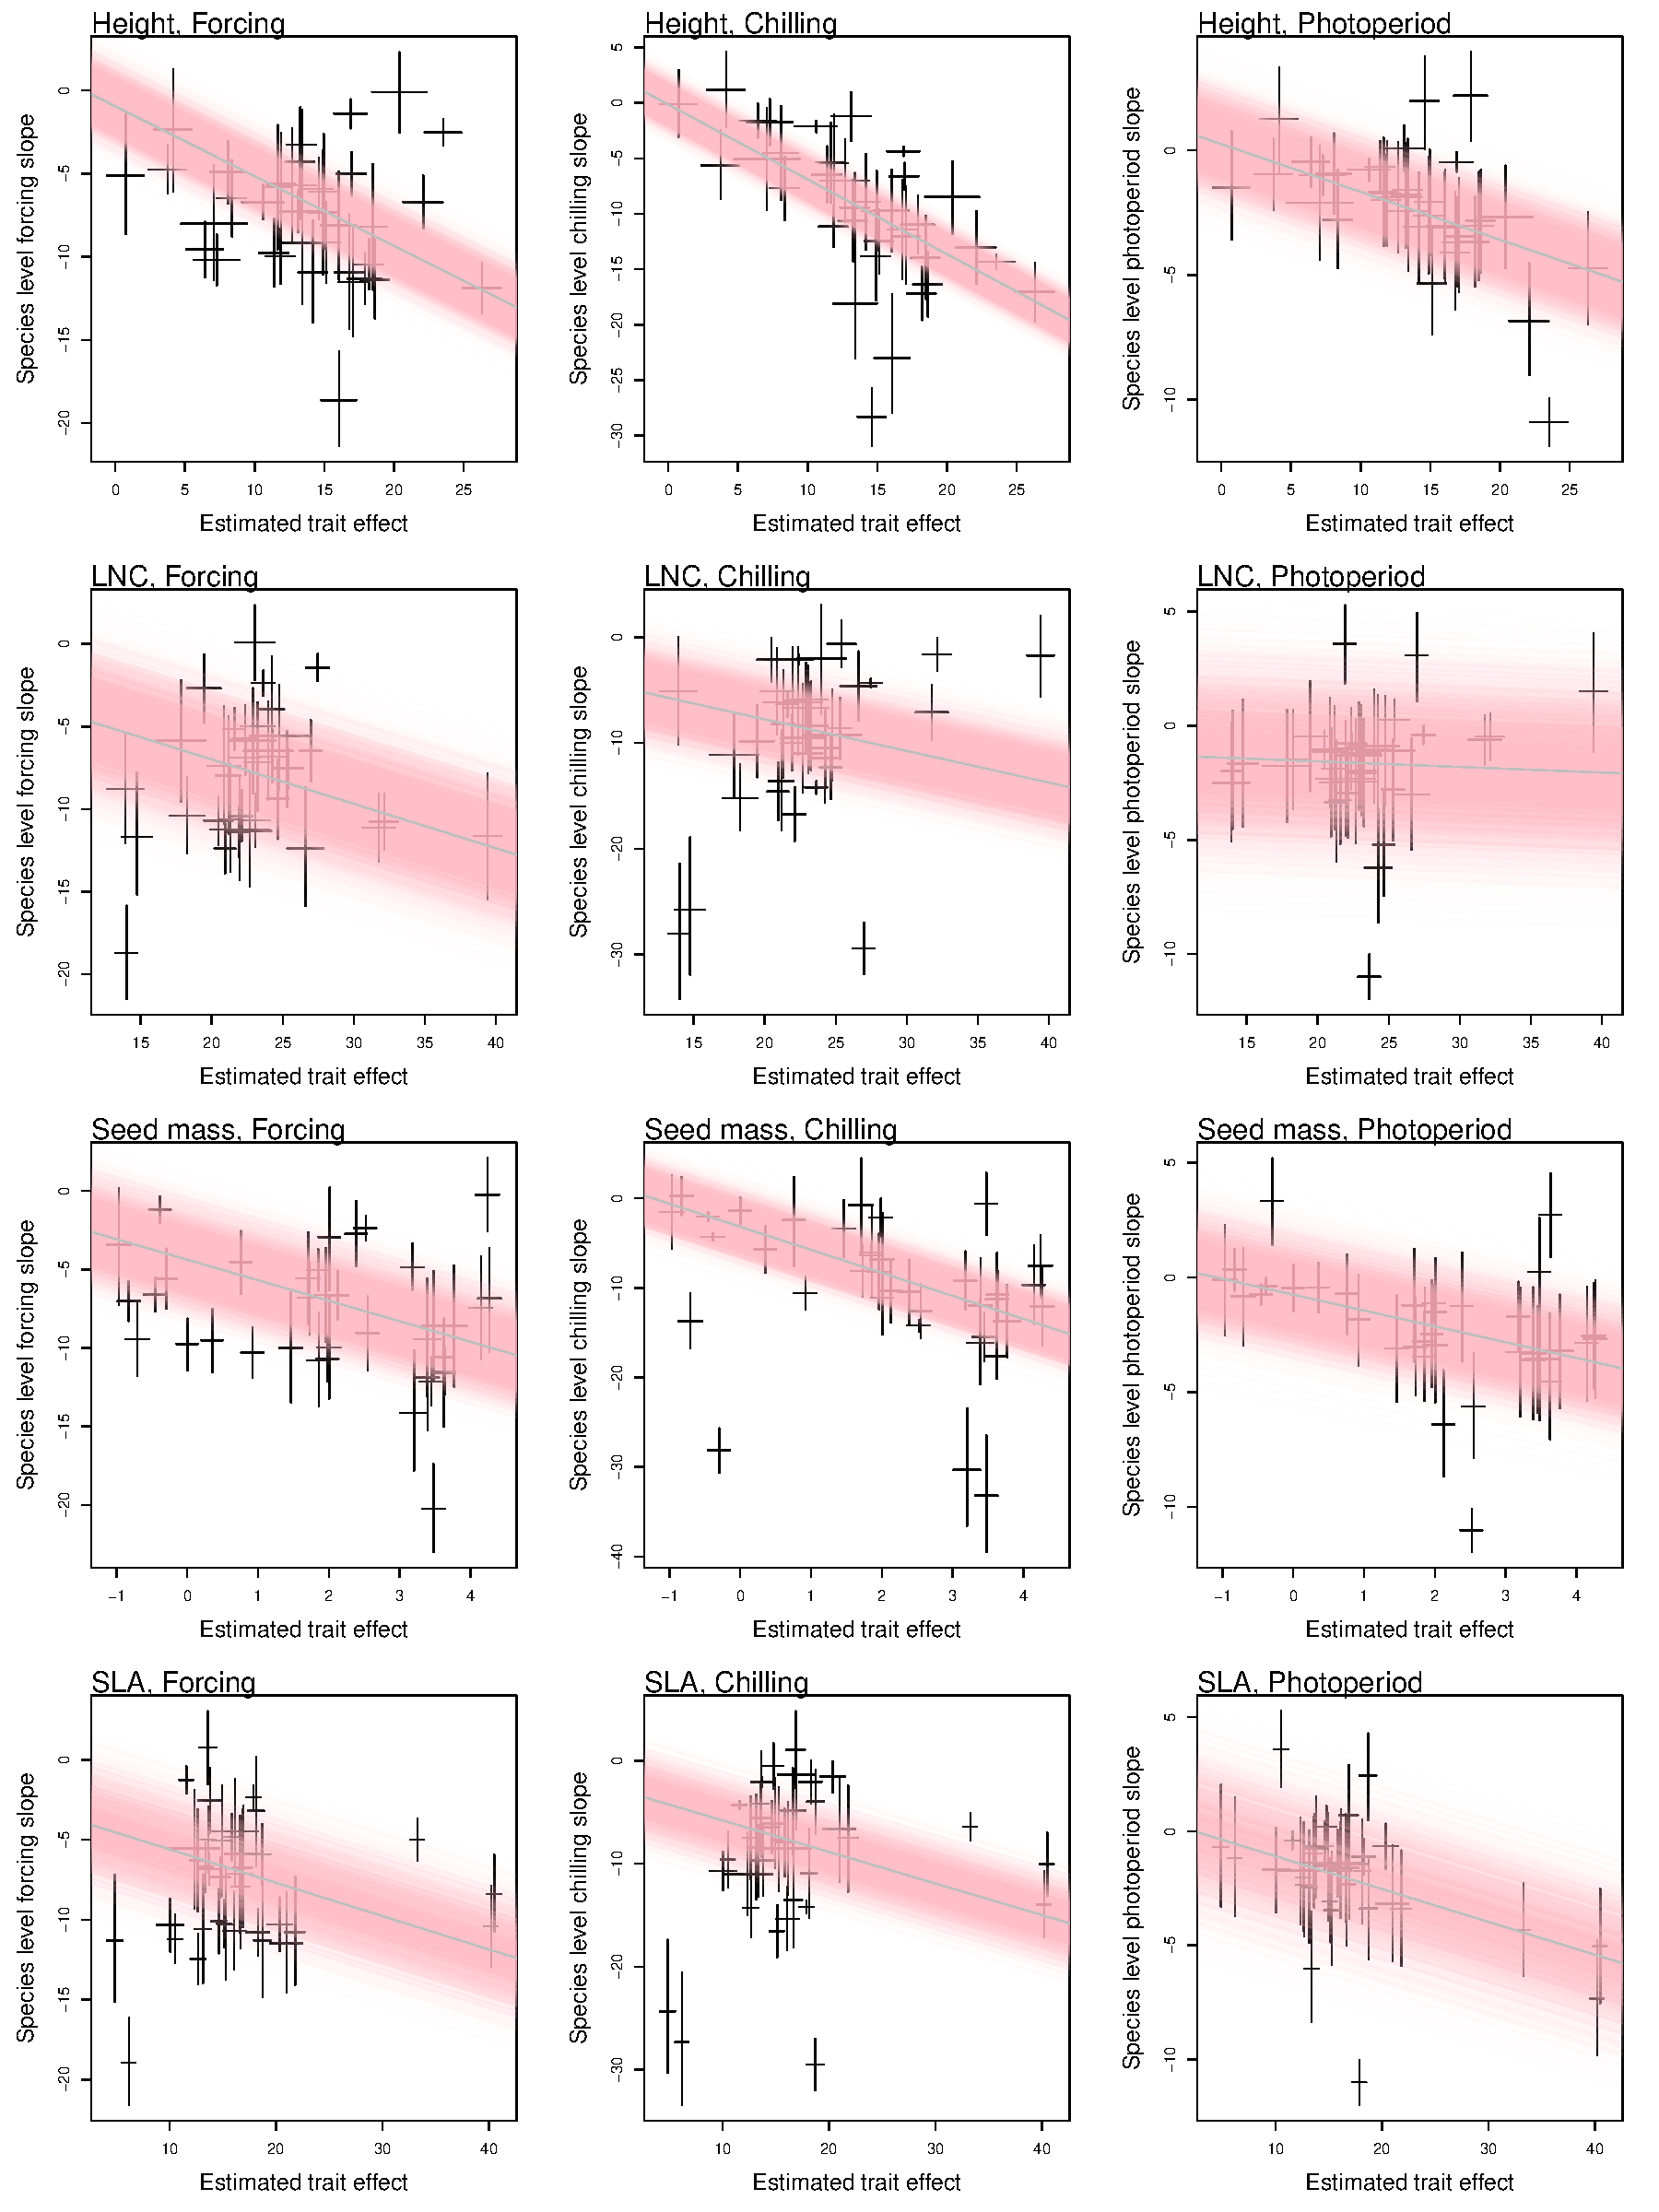
\includegraphics[width=\textwidth]{..//..//analyses/traits/figures/cuetrait_wtrend.pdf} 
    \caption{Trait relationships with cue slopes}
    \label{fig:cuetraits_wtrend}
\end{figure}


We found that as SLA increased, responses to each cue generally became more negative. Chilling had the largest trait slope in response to SLA at -9.3 (90\% uncertainty interval: -17.9, -18.1), followed by the forcing slope at -7.8 (90\% uncertainty interval: -14.5, -10.5), the photoperiod slope at -2.0 (90\% uncertainty interval: -11.1, -11.6). At hight SLA values, such as those of leaves from \textit{Fagus grandifolia}, this negative trait effect produces a more negative slope in the full model relative to the slope when the trait effect is set to zero. There is a much smaller difference in the slopes of species that produces leaves with low SLA, such as \textit{Quercus ilex} \ref{fig:sla}. The relatively small trait effect of photoperiod is reflected in the smaller difference in the slopes between the full model and the cue only model \ref{fig:sla}. Furthermore, the relationship between trait effects and estimated model slopes was negative for each of the cues, indicating that larger trait values are correlated with more negative slope estimates \ref{fig:cuetraits}. 

In modeling relationship between species height and cue responses, we found that as tree height increased cue responses became more negative. Chilling had the largest trait slope in response to height at -9.6 (90\% uncertainty interval: -14.6, -20.8), followed by the forcing slope at -7.5 (90\% uncertainty interval: -12.1, -10.7), the photoperiod slope at -2.3 (90\% uncertainty interval: -7.8, -12.4). This means that the estimated slopes for a tall tree, such as \textit{Acer pseudoplantanus}, could change from having a positive slope when the trait effect is zero, to having a negative slope in response to chilling and forcing cues \ref{fig:slopes}. The change in slope in response to photoperiod is follows a similar trend, becoming more negative when the trait effect is included, but is more moderate in magnitude. In general, taller tree species, for which there is a greater estimated trait effect,  also have more negative estimated slopes for each of the three cues \ref{fig:cuetraits}. 

In our model of LNC, we found species that produce leaves with hight LNC also had increasingly negative cue responses. Chilling had the largest trait slope in response to LNC at -9.6 (90\% uncertainty interval: -16, -19.1), followed by the forcing slope at -8.1 (90\% uncertainty interval: -12.9, -10.7), the photoperiod slope at -1.7 (90\% uncertainty interval: -8.2, -12.3). Species like \textit{Alnus glutinosa} that have high LNC would have a more negative slope in response to increasing forcing and chilling cues, while species with low LNC like \textit{Quercus ilex} experience a much smaller decrease in their slopes \ref{fig:slopes}. The model estimated trait effect of LNC for photoperiod is relatively negligible, producing no noticeable differences between the cue only slopes and full model slope.  The effects of LNC and estimated model slopes were negatively correlated for each of the cues, indicating that species with higher LNC have a stronger negative response to increasing cues \ref{fig:cuetraits}. 

Finally, we found that species with increasingly large seeds also had more negative responses to cues when trait effects were incorporated. Chilling had the largest trait slope in response to seed mass at -10 (90\% uncertainty interval: -15.3, -19.4), followed by the forcing slope at -8 (90\% uncertainty interval: -12.2, -10.3), the photoperiod slope at -2.2 (90\% uncertainty interval: -7.9, -12.2). Our model estimates for the model cue slopes were all negative, however, given the nature of the log10 transformation of the seed mass data, the modelled response has a positive slope for species with large seeds. This is shown for \textit{Aesculus hippocastanum} in \ref{fig:slopes}, where we found the negative effect of seed mass to make the slopes more negative for each of the cues. The magnitude of the differences between the cue only slopes and full model slopes are much greater for forcing and chilling cues and relatively moderate for photoperiod. As we observed for the other traits, species with larger seeds had larger trail effects, which were again negatively correlated with the estimates cue slopes \ref{fig:cuetraits}
%In line with our our prediction, the high SLA species had earlier budburst dates than the low SLA species.\\

Geoff : "Overall, we found that conservative species, which generally had high traits values for SLA, Height, etc., shifted their phenology more and earlier in response to forcing, chilling, and photoperiod, than acquisitive species with low trait values. This responsiveness is linked to later budbursting - earlier sp have lower slopes bc they require less cues in general, having a lower intercept"


\begin{figure}[h!]
    \centering
 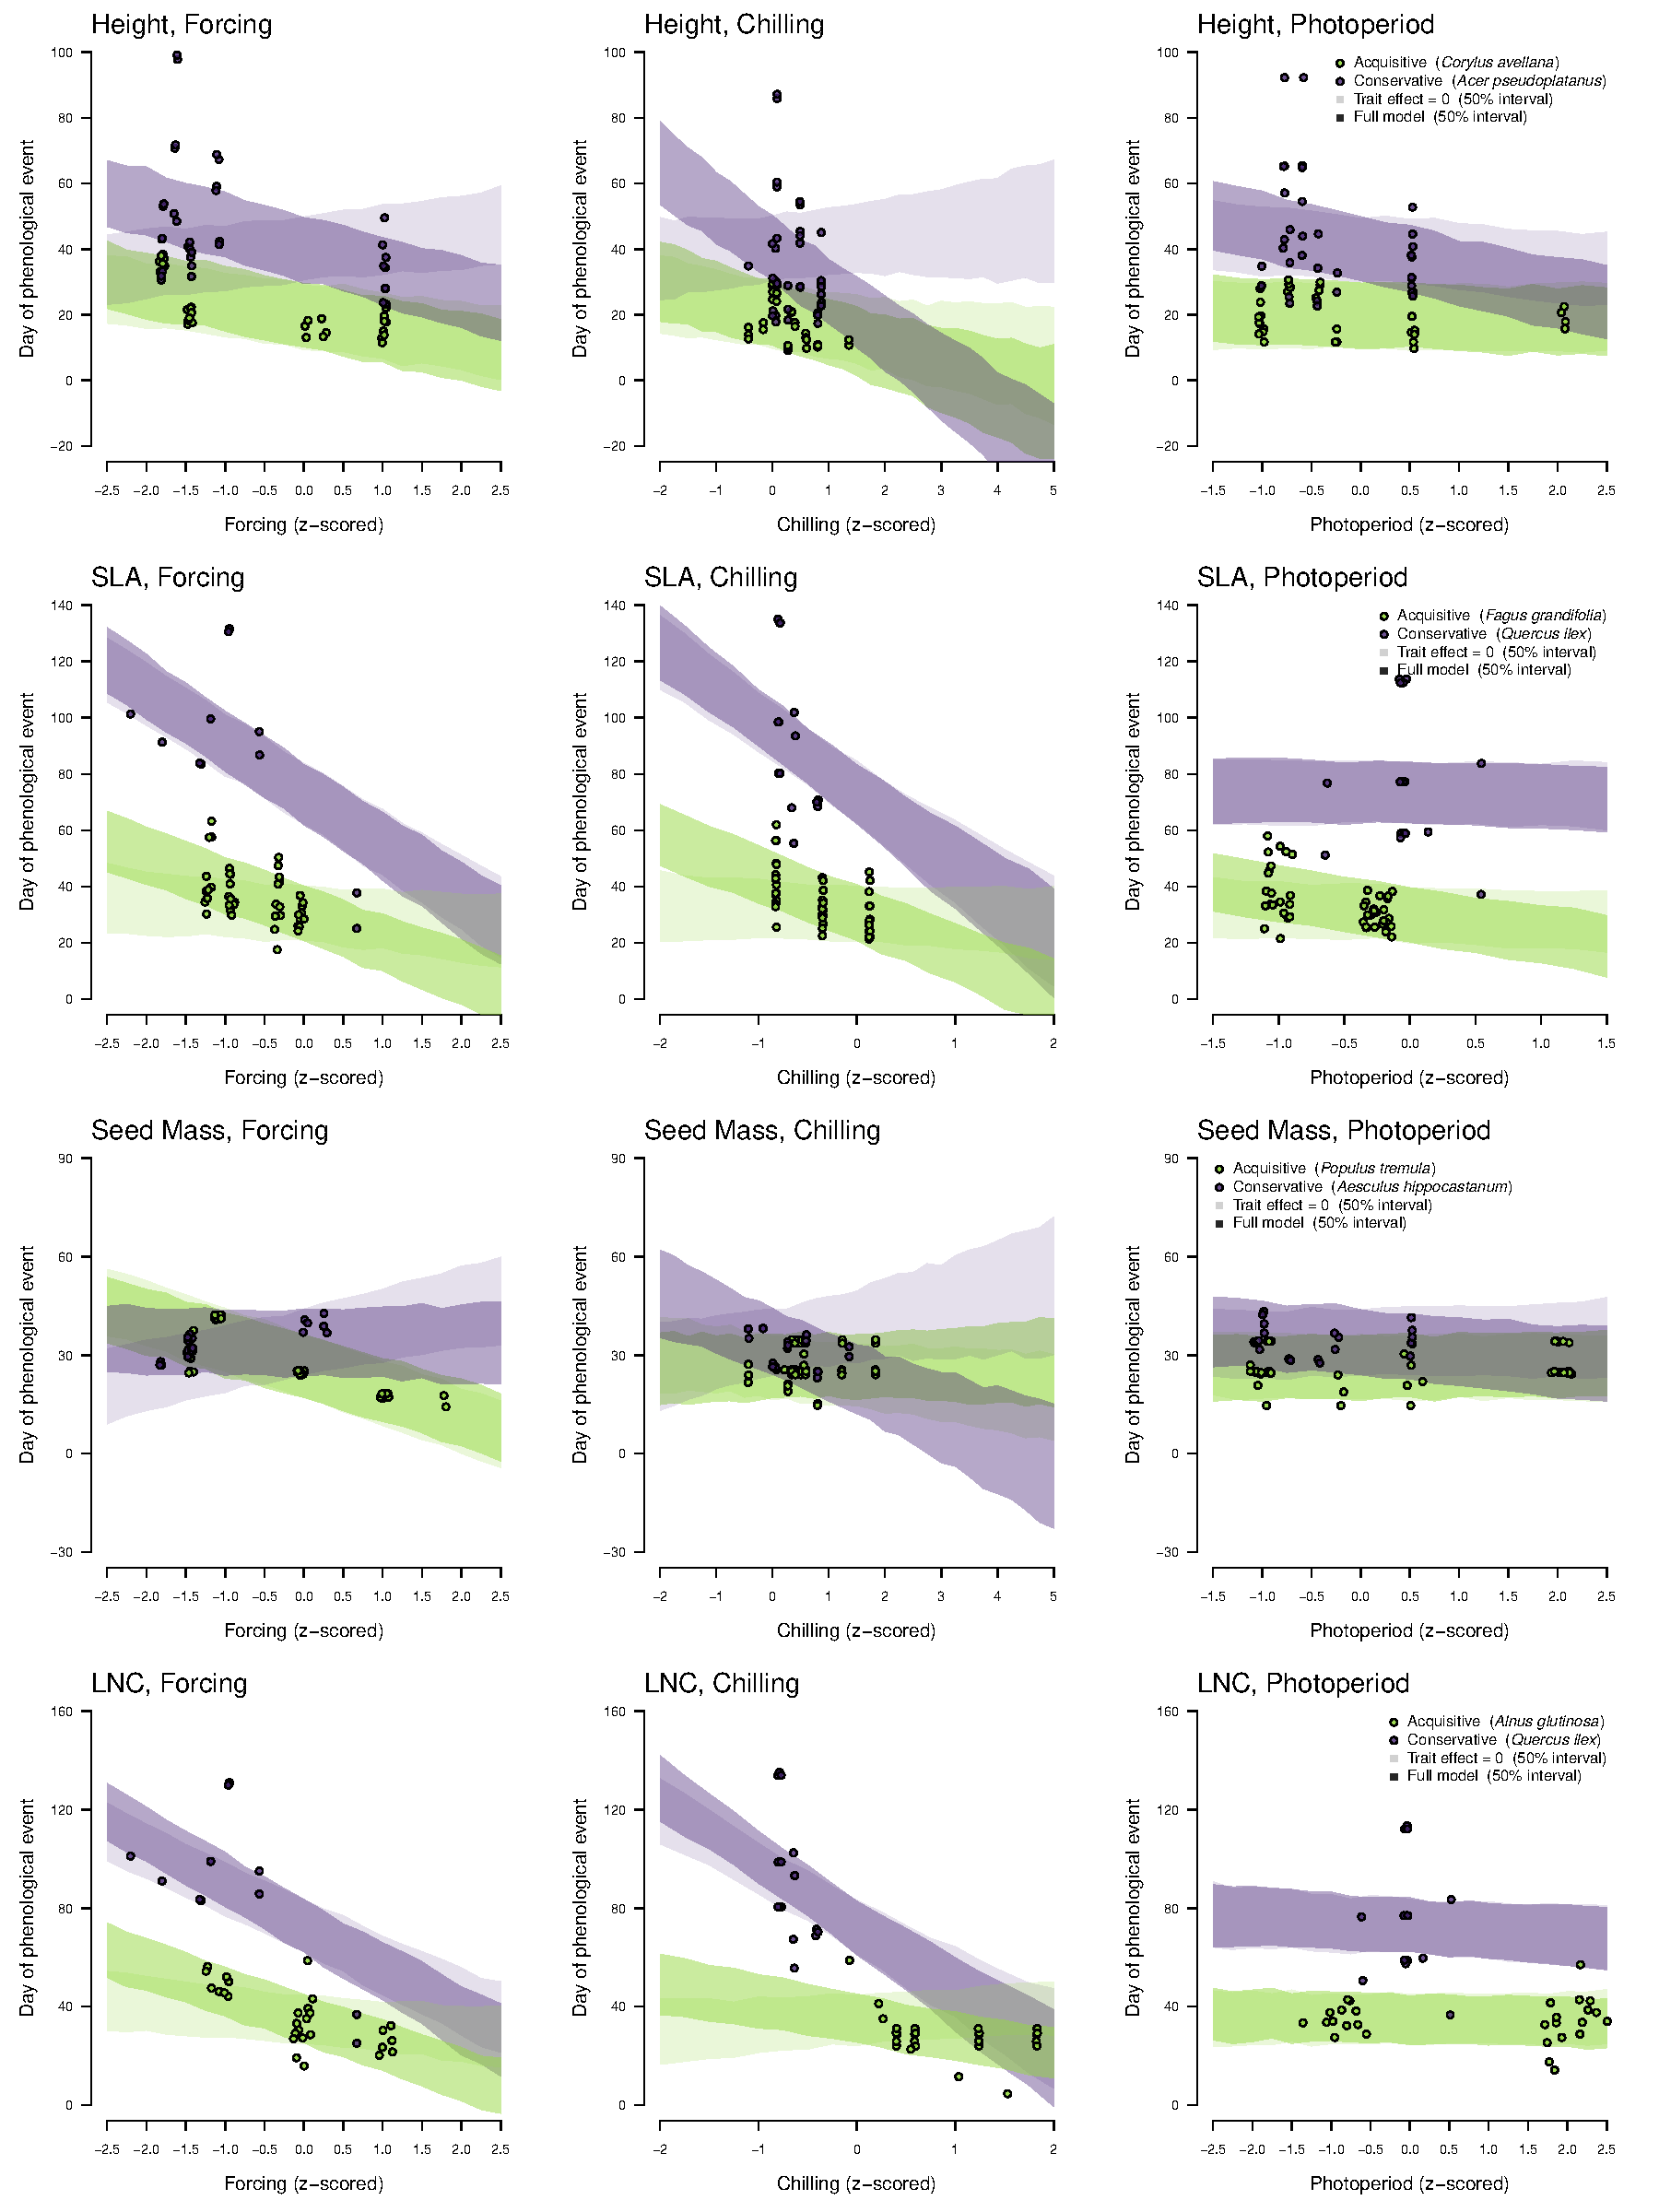
\includegraphics[width=\textwidth]{..//..//analyses/traits/figures/slopesConsAcqu.pdf} 
    \caption{Estimated cue responses for acquisitive and conservative spp.}
    \label{fig:slopes}
\end{figure}


%need to redo the pgls analysis
PGLS suggests there are no strong phylogenetic effects for most of our cue trait relationshps, with the exception of .... This suggests there is a phylogenetic effect influencing the cue response of species for these traits. Given the complexity of our model, however, we were not able to fully incorporate these phylogenetic effects into our current analysis. 

\section{Discussion}

Discuss the DF paper again 

\begin{itemize}
\item What do our results suggest for the relationship between cue use and traits? 
- Species responses to forcing, chilling, and photoperiod cues are influenced by species functional traits. 
- generally in line with previous studies of phenological cues, cue responses were all negative leading to strong advances in bb date 
	\begin{itemize}
	\item Do we find relationships between cues and traits?
	- yes, with the exception of LNC and photoperiod, all traits had an effect of the response of species to cues
	\item Do these trends agree with an acquisitive/conservative tradeoff?
	- yes, with the exception of seed mass, species with traits associated with acquisitive growth strategies did budburst earlier
	\end{itemize}
\item How do our results relate to previous studies? 
        Huang et al. 2018 - found several growth strategies - all combinations of early- fast, early-slow, late-fast etc - but looked at flowering
        Osada 2017 - bb later for sp with greater LMA, thickness, Narea – driven by differences across deciduous and evergreen spp; 	Deciduous alone: bb positively correlated with leaf mass, area, vessel diam in cross spp comparisons
\item What do our results suggest for the bigger picture?
Sun, S., D. Jin, and R. Li. 2006. LMA neg correl with leafout; larger LMA = earlier
	\begin{itemize}
	\item How might traits constrain/facilitate future shifts in phenology?
	- our findings do partially (maybe not LNC and Seedmass) support the idea that phenology is an important functional trait
	\item How might ecosystem functioning shift if species track temperature? How to our results relate to seasonality and frost risk?
	\item What does it mean if more competitive/invasive species respond to warming and start bb earlier - outcompete species and lead to compressed temporal niche?
	\item Relate our results to invasion success 
	\end{itemize}

\item Limitations/strengths?
	\begin{itemize}
	\item we assume stronger cues mean earlier bb but really it's more complicated than this
	\item broad approach means lose detail and compromise - traits come from different populations to the phenology data
	\item disconnect between trait data - observational - and phenology data that is in a controlled environment
	\item limited data may have reduced diversity of traits/strategies - may not be enough to detect predicted trends -- reframe this as less of a limitation and more of a future direction
   \item Why we think mean height values were different from geometric mean values for some species. Talk about the influence of accounting for the study effect. 
	\end{itemize}
\end{itemize}


\pagebreak
\bibliographystyle{refs/bibstyles/amnat.bst}% 
\bibliography{refs/traitors.bib}



\end{document}